\section{Architecture}

The trace logs read by PET can easily grow to 10s of gigabytes. Due to memory
constraints on commonly available computers, it is not feasible to read the
entire log file into memory and then start parsing. One of PET's major design
goals is to be user friendly and convenient to use, and as a consequence it must
be reasonably fast. To gain speed, the PET core is built around a parallel
pattern similar to MapReduce \cite{dean2008mapreduce}.


\subsection{Overview}

\begin{figure}[ht]
    \includegraphics[width=\textwidth]{figs/pet-pipeline-gv.pdf}
    \caption{How PET works.}
    \label{fig:pipeline}
\end{figure}

In order to obtain acceptable performance, we have looked at different ways of
digesting large data sets. The final implementation of PET follows a scheme
borrowing ideas from the producer-consumer pattern as explained by Gamma et. al.
in \cite{designpatterns} and the MapReduce algorithm. As depicted in
\autoref{fig:pipeline}, this scheme makes it rather easy to let a producer
(sequentially) read the lines from the log file into ring buffers (produce) and
let multiple consumers pick from their ring buffer (consume). Each consumer
parses the log lines they pick, and apply the weight of each read event to their
result vector (map). When all lines are read and parsed, the result vectors are
merged (reduce) and idle-task power and static power consumption is added. This
combination of algorithms allows PET to take advantage of as many cores as
possible, only limited by the hard drive data transfer rate.

The next subsections will describe in detail the most important parts of the
workflow, in sequential order. For further understanding of the program flow, a
call graph is seen in \autoref{fig:callgraph}.

\begin{figure}
    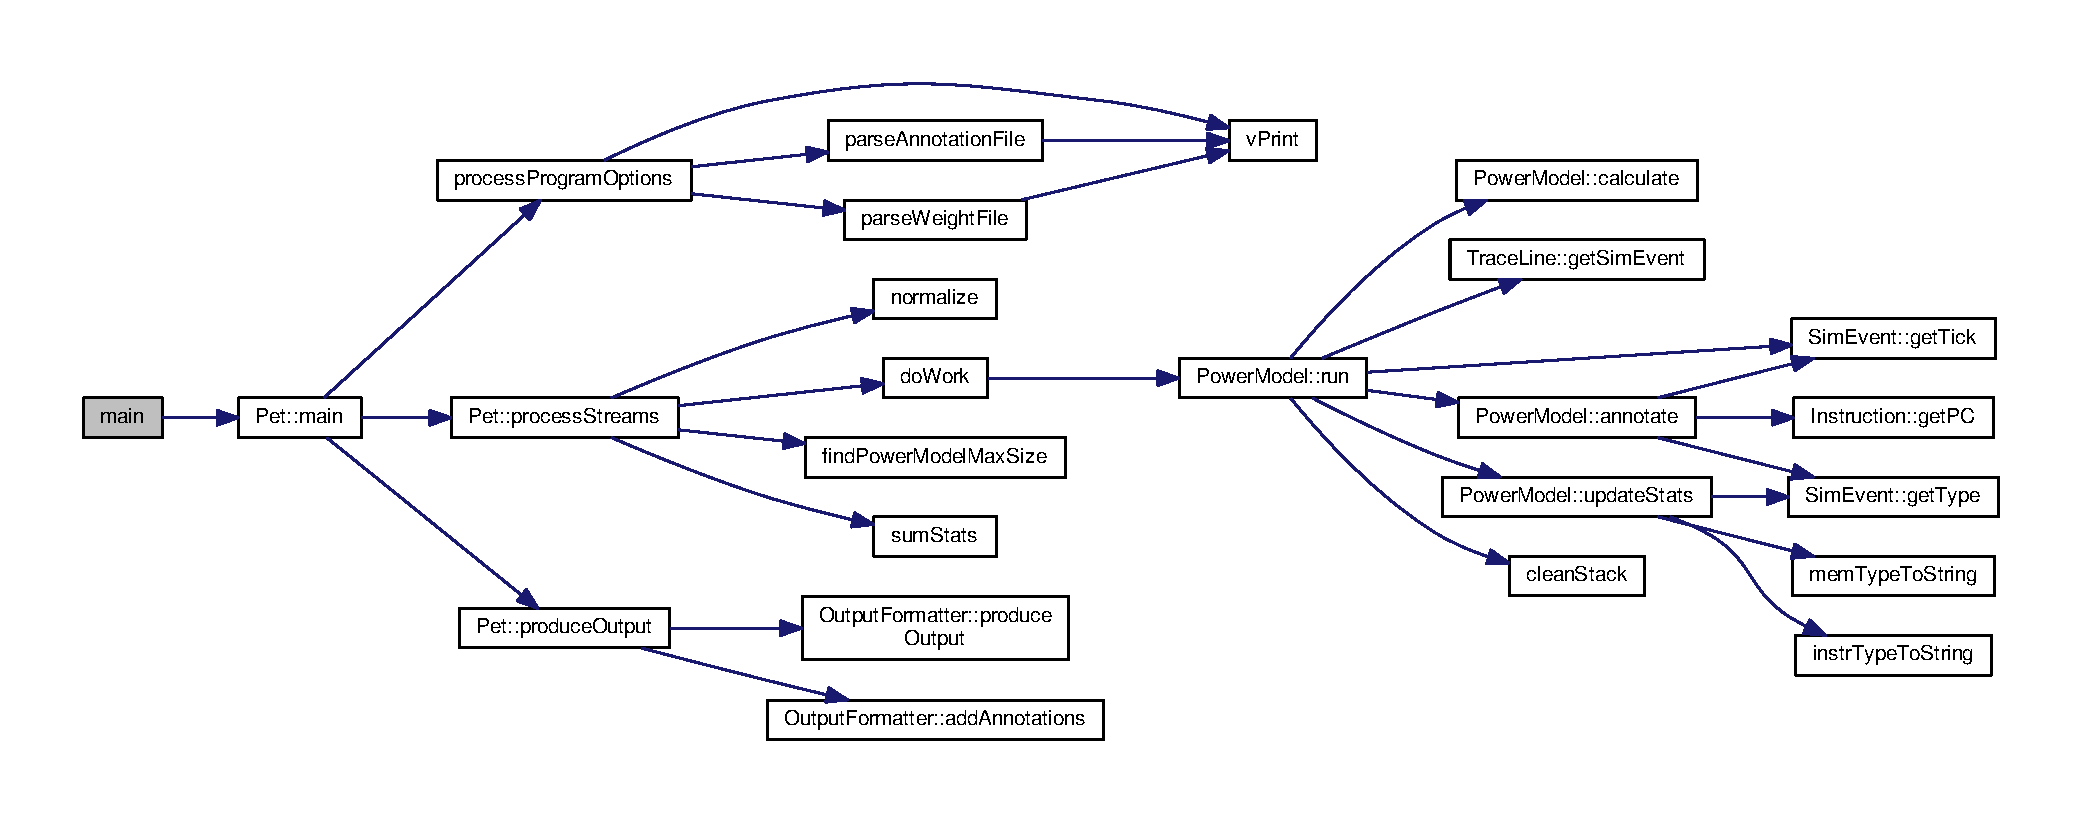
\includegraphics[width=\textwidth]{figs/maincallgraph.pdf}
    \caption{Call graph.}
    \label{fig:callgraph}
\end{figure}


\subsection{Argument Parsing and Program Options}

As any other non-trivial programs, PET has to adapt to input options given from
the command line or from a settings file. PET makes extensive use of the
\texttt{Boost} library and utilize \texttt{Boost::Program\_options} for parsing
the command line. This allows easy extraction of program options, both with long
(\texttt{\textemdash \textemdash option=\emph{value}}) and short
(\texttt{\textemdash o~\emph{value}}) option style.


\subsection{Reading Trace Logs}

When arguments are parsed and a trace log has been specified, either by path or
as \texttt{stdin}, a single thread is kicked off reading each line of the log
file into a C++ string container. This happens in the
\texttt{Pet::processStreams} class member function seen in \autoref{fig:callgraph}. The string
container is then inserted into one of many circular buffers. The circular
buffers are implemented with \texttt{boost::lockfree::spsc\_queue}, a lock-free
single producer, single consumer queue. The property of being lock-free is
explained by Tim Blechmann in \cite{boostlockfree}:

\begin{quote}
    Data structures are \emph{lock-free}, if some concurrent operations
are guaranteed to be finished in a finite number of steps. While it is in theory
possible that some operations never make any progress, it is very unlikely to
happen in practical applications.
\end{quote}

In PET, this queue has a fixed size of 8192~elements, but dynamic size is also
available in the library implementation. Which buffer the string is inserted
into is determined by a simple circular algorithm; the next ring buffer is
selected when the current one is full. When the buffers are small, each are
filled fast enough to keep all workers occupied. We observed that this method
avoids locking better than using a single ring buffer shared by all worker
threads. The number of threads and the size of the ring buffers are tightly
coupled with how fast the host computer is able to feed PET with the log files.


\subsection{String to Event Mapping and Power Accumulation}

String parsing and mapping are the most compute-intensive parts of PET.
PET spawns multiple worker threads as specified by the user. As the producer
fills the ring buffers for each of the workers, the workers pick strings from
their pool. The strings are popped from the ring buffer, thus making space for
new elements right away. Each string is parsed by the \texttt{TraceLine} class,
which looks for patterns in the strings containing known event types. When
connecting PET with gem5, the trace logs as previously seen \autoref{lst:trace}
contains an event type designation in the second colon-separated column. The
\texttt{TraceLine} class extracts this part by string trimming.

The event types are instantiated as objects of their parent type (Instruction-
or Memory-event). The right parameters are found from progressive string
parsing. If the event is unrecognized, a dummy object of type
\texttt{UnknownEvent} is returned. This type has zero cost later in the reduce
phase. Each event object is able to figure out its own weight as written in the
\emph{weights}-file. After the event has been parsed, the weight is added to the
power model at the corresponding time step.

In order to reduce the time used for disposal of the string objects after they
are parsed, they are placed in a static-size array. When this array is full, or
the ring buffer is empty, the worker frees all the string data. This helps
keeping the memory footprint low while avoiding unnecessary calls to
\texttt{free()}. This optimization does not have a massive impact on
performance, but as can be seen from \cite{kernighan1988c}, the \texttt{free()}
implementation contains enough pointer arithmetic to make a difference in a
tight loop.


\subsection{Data Reduction}

When all lines from the trace log have been consumed by the workers, the threads
are joined and their data is returned as standard C++ vectors. These vectors are
further wrapped in yet another standard C++ vector. The inner vectors are then
combined; the value from the corresponding buckets in each vector is added
together and put in a result vector. This reduction happens as the last part of
\texttt{Pet::processStreams}, as seen in \autoref{fig:callgraph}.

After this reduction, the number of idle cycles is estimated by subtracting
recorded events from the maximum number of events in a bucket. This is done more
simplistic than accurate using \autoref{eq:idle}. \texttt{eventsInWorkerBucket}
is the number of events recorded in each vector at each bucket, and each event
is pinned to the cycle where it originated. Note that N is the number of worker
threads, not the number of buckets.

\begin{equation}
    eventsInBucket = \sum_{n=1}^{N} eventsInWorkerBucket_n
\end{equation}

\begin{equation}
    idleEvents = \frac{ticksInBucket}{ticksInCycle} - eventsInBucket
\label{eq:idle}
\end{equation}

It should also be noted that even though this method might work well in a
single-cycle in-order CPU, the out-of-order nature of the Cortex-A9 makes it
hard to tell how many idle cycles actually occurred. E.g., a single cycle may fill
the pipeline with four events, then idle the three next cycles; this would be
calculated as no idle time. When the approximate numbers of \texttt{idleEvents}
have been estimated, that number is multiplied by the \emph{Idle}-weight and
added to the sum in the result vector. Finally, the entire vector is normalized
according to bucket size and then static current drain is added.


\subsection{Output Production and Annotations}

After the result vector has been completely accumulated, annotation is added to
a new vector in the same manner as the data reduction. With the new, merged
annotation map containing all last matches between a symbol and the program
counter within each measure point, this map is fed to the
\texttt{OutputProducer} object as seen in \autoref{fig:callgraph}. The
\texttt{OutputProducer} is responsible for generating output as defined by the
input arguments. Its options have already been described in
\autoref{sec:output}, and its implementation is a simple nested if-else-clause
that calls internal functions for each output type. The graphical output is
produced using a wrapper around \texttt{gnuplot}, while the textual outputs are
created by \texttt{printf}-statements.


\subsection{Unit Tests}

All internal string parsing is verified by unit tests. The unit tests
are written with help from the Boost Test Library \cite{boostunittest}.

The test library generates a new binary with the same program content, except the
main function, thus the program flow is different. The test binary will
run through the listed functions with a certain input, and if the output is unexpected,
the test binary will print to the console an error message containing a description of what
went wrong.

